% Created by tikzDevice version 0.12 on 2019-04-11 07:16:30
% !TEX encoding = UTF-8 Unicode
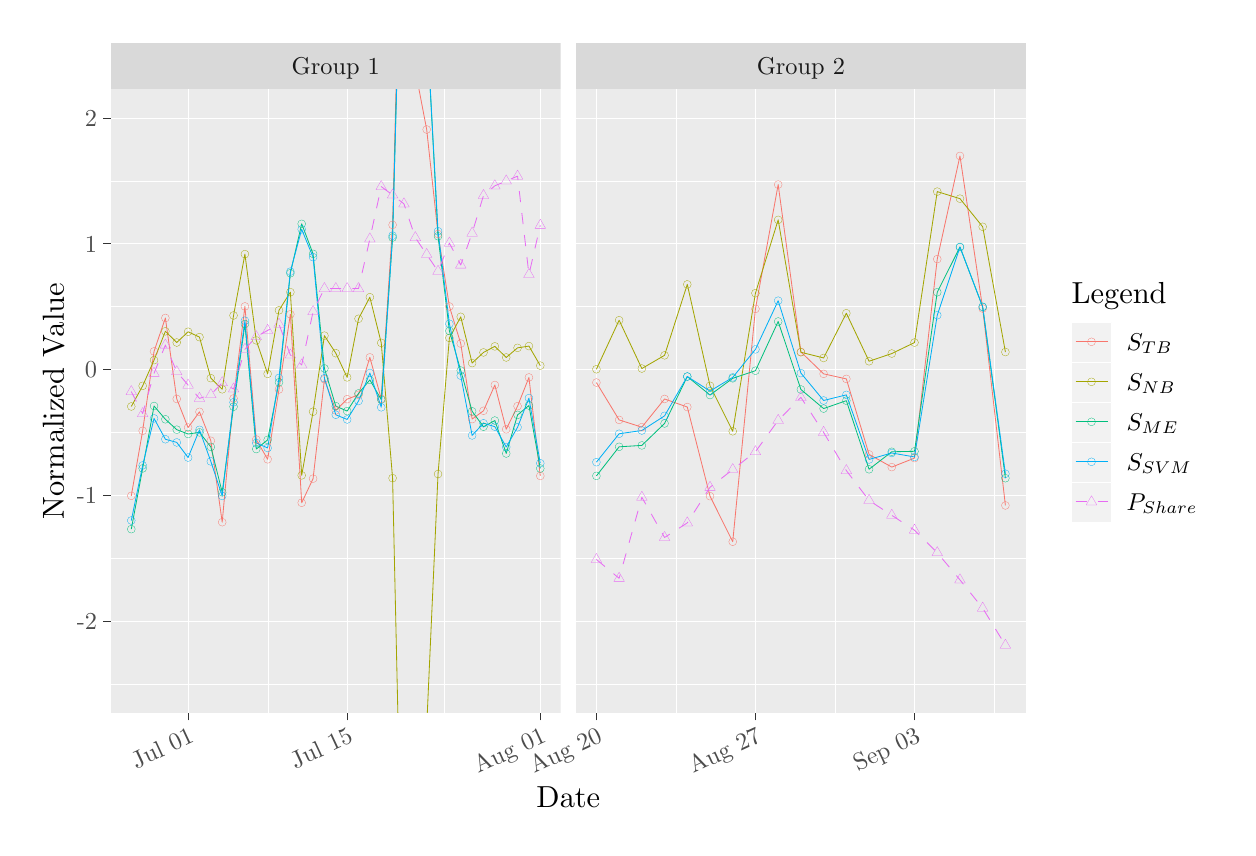
\begin{tikzpicture}[x=1pt,y=1pt]
\definecolor{fillColor}{RGB}{255,255,255}
\path[use as bounding box,fill=fillColor,fill opacity=0.00] (0,0) rectangle (433.62,289.08);
\begin{scope}
\path[clip] (  0.00,  0.00) rectangle (433.62,289.08);
\definecolor{drawColor}{RGB}{255,255,255}
\definecolor{fillColor}{RGB}{255,255,255}

\path[draw=drawColor,line width= 0.1pt,line join=round,line cap=round,fill=fillColor] (  0.00,  0.00) rectangle (433.62,289.08);
\end{scope}
\begin{scope}
\path[clip] ( 30.06, 41.55) rectangle (192.62,266.77);
\definecolor{fillColor}{gray}{0.92}

\path[fill=fillColor] ( 30.06, 41.55) rectangle (192.62,266.77);
\definecolor{drawColor}{RGB}{255,255,255}

\path[draw=drawColor,line width= 0.1pt,line join=round] ( 30.06, 51.79) --
	(192.62, 51.79);

\path[draw=drawColor,line width= 0.1pt,line join=round] ( 30.06, 97.29) --
	(192.62, 97.29);

\path[draw=drawColor,line width= 0.1pt,line join=round] ( 30.06,142.79) --
	(192.62,142.79);

\path[draw=drawColor,line width= 0.1pt,line join=round] ( 30.06,188.29) --
	(192.62,188.29);

\path[draw=drawColor,line width= 0.1pt,line join=round] ( 30.06,233.79) --
	(192.62,233.79);

\path[draw=drawColor,line width= 0.1pt,line join=round] ( 86.71, 41.55) --
	( 86.71,266.77);

\path[draw=drawColor,line width= 0.1pt,line join=round] (150.34, 41.55) --
	(150.34,266.77);

\path[draw=drawColor,line width= 0.1pt,line join=round] ( 30.06, 74.54) --
	(192.62, 74.54);

\path[draw=drawColor,line width= 0.1pt,line join=round] ( 30.06,120.04) --
	(192.62,120.04);

\path[draw=drawColor,line width= 0.1pt,line join=round] ( 30.06,165.54) --
	(192.62,165.54);

\path[draw=drawColor,line width= 0.1pt,line join=round] ( 30.06,211.04) --
	(192.62,211.04);

\path[draw=drawColor,line width= 0.1pt,line join=round] ( 30.06,256.54) --
	(192.62,256.54);

\path[draw=drawColor,line width= 0.1pt,line join=round] ( 57.97, 41.55) --
	( 57.97,266.77);

\path[draw=drawColor,line width= 0.1pt,line join=round] (115.44, 41.55) --
	(115.44,266.77);

\path[draw=drawColor,line width= 0.1pt,line join=round] (185.23, 41.55) --
	(185.23,266.77);
\definecolor{drawColor}{RGB}{248,118,109}

\path[draw=drawColor,line width= 0.3pt,line join=round] ( 37.44,119.92) --
	( 41.55,143.42) --
	( 45.66,172.11) --
	( 49.76,184.17) --
	( 53.87,154.92) --
	( 57.97,144.57) --
	( 62.08,150.26) --
	( 66.18,139.79) --
	( 70.29,110.39) --
	( 74.39,155.10) --
	( 78.50,188.35) --
	( 82.60,140.26) --
	( 86.71,133.11) --
	( 90.81,158.35) --
	( 94.92,185.51) --
	( 99.02,117.40) --
	(103.13,126.12) --
	(107.23,162.04) --
	(111.34,150.77) --
	(115.44,154.84) --
	(119.55,156.40) --
	(123.65,169.94) --
	(127.76,154.96) --
	(131.86,217.82) --
	(133.67,289.08);

\path[draw=drawColor,line width= 0.3pt,line join=round] (139.48,289.08) --
	(140.07,273.75) --
	(144.18,252.28) --
	(148.28,214.52) --
	(152.39,188.33) --
	(156.49,174.93) --
	(160.60,147.64) --
	(164.71,150.64) --
	(168.81,159.95) --
	(172.92,143.97) --
	(177.02,152.32) --
	(181.13,162.69) --
	(185.23,127.10);
\definecolor{drawColor}{RGB}{163,165,0}

\path[draw=drawColor,line width= 0.3pt,line join=round] ( 37.44,152.20) --
	( 41.55,159.65) --
	( 45.66,168.95) --
	( 49.76,179.37) --
	( 53.87,175.31) --
	( 57.97,179.19) --
	( 62.08,177.26) --
	( 66.18,162.43) --
	( 70.29,158.41) --
	( 74.39,185.09) --
	( 78.50,207.25) --
	( 82.60,176.09) --
	( 86.71,163.98) --
	( 90.81,186.95) --
	( 94.92,193.51) --
	( 99.02,127.31) --
	(103.13,150.31) --
	(107.23,177.79) --
	(111.34,171.46) --
	(115.44,162.71) --
	(119.55,183.89) --
	(123.65,191.69) --
	(127.76,175.18) --
	(131.86,126.30) --
	(134.69,  0.00);

\path[draw=drawColor,line width= 0.3pt,line join=round] (138.83,  0.00) --
	(140.07, 24.90) --
	(144.18, 36.46) --
	(148.28,127.79) --
	(152.39,176.97) --
	(156.49,184.59) --
	(160.60,167.88) --
	(164.71,171.73) --
	(168.81,173.92) --
	(172.92,169.91) --
	(177.02,173.38) --
	(181.13,174.02) --
	(185.23,166.95);
\definecolor{drawColor}{RGB}{0,191,125}

\path[draw=drawColor,line width= 0.3pt,line join=round] ( 37.44,107.87) --
	( 41.55,129.82) --
	( 45.66,152.37) --
	( 49.76,147.57) --
	( 53.87,143.82) --
	( 57.97,142.25) --
	( 62.08,142.84) --
	( 66.18,137.59) --
	( 70.29,121.20) --
	( 74.39,152.11) --
	( 78.50,181.99) --
	( 82.60,136.82) --
	( 86.71,140.12) --
	( 90.81,160.93) --
	( 94.92,200.35) --
	( 99.02,218.19) --
	(103.13,207.35) --
	(107.23,165.96) --
	(111.34,152.32) --
	(115.44,150.53) --
	(119.55,156.93) --
	(123.65,161.80) --
	(127.76,154.67) --
	(131.86,213.24) --
	(133.86,289.08);

\path[draw=drawColor,line width= 0.3pt,line join=round] (144.28,289.08) --
	(148.28,213.72) --
	(152.39,179.50) --
	(156.49,165.17) --
	(160.60,150.46) --
	(164.71,144.87) --
	(168.81,147.11) --
	(172.92,135.21) --
	(177.02,149.15) --
	(181.13,152.55) --
	(185.23,129.80);
\definecolor{drawColor}{RGB}{0,176,246}

\path[draw=drawColor,line width= 0.3pt,line join=round] ( 37.44,110.99) --
	( 41.55,130.91) --
	( 45.66,147.89) --
	( 49.76,140.36) --
	( 53.87,139.21) --
	( 57.97,133.74) --
	( 62.08,143.75) --
	( 66.18,132.35) --
	( 70.29,119.87) --
	( 74.39,153.72) --
	( 78.50,183.18) --
	( 82.60,139.00) --
	( 86.71,137.21) --
	( 90.81,162.52) --
	( 94.92,200.93) --
	( 99.02,216.21) --
	(103.13,206.15) --
	(107.23,162.41) --
	(111.34,149.20) --
	(115.44,147.51) --
	(119.55,154.18) --
	(123.65,164.29) --
	(127.76,151.90) --
	(131.86,213.92) --
	(133.94,289.08);

\path[draw=drawColor,line width= 0.3pt,line join=round] (144.28,289.08) --
	(148.28,215.52) --
	(152.39,182.07) --
	(156.49,163.33) --
	(160.60,141.74) --
	(164.71,146.14) --
	(168.81,144.90) --
	(172.92,137.55) --
	(177.02,144.69) --
	(181.13,155.24) --
	(185.23,131.68);
\definecolor{drawColor}{RGB}{231,107,243}

\path[draw=drawColor,line width= 0.3pt,dash pattern=on 4pt off 4pt ,line join=round] ( 37.44,157.57) --
	( 41.55,149.63) --
	( 45.66,164.18) --
	( 49.76,174.39) --
	( 53.87,164.75) --
	( 57.97,159.93) --
	( 62.08,155.11) --
	( 66.18,156.44) --
	( 70.29,160.78) --
	( 74.39,158.51) --
	( 78.50,172.88) --
	( 82.60,177.41) --
	( 86.71,179.68) --
	( 90.81,181.95) --
	( 94.92,170.80) --
	( 99.02,167.21) --
	(103.13,186.48) --
	(107.23,194.80) --
	(111.34,194.80) --
	(115.44,194.80) --
	(119.55,194.80) --
	(123.65,212.75) --
	(127.76,231.65) --
	(131.86,228.62) --
	(135.97,225.41) --
	(140.07,213.22) --
	(144.18,207.13) --
	(148.28,201.03) --
	(152.39,211.24) --
	(156.49,203.30) --
	(160.60,214.83) --
	(164.71,228.43) --
	(168.81,231.93) --
	(172.92,233.68) --
	(177.02,235.43) --
	(181.13,199.90) --
	(185.23,217.66);
\definecolor{drawColor}{RGB}{248,118,109}

\path[draw=drawColor,line width= 0.1pt,line join=round,line cap=round] ( 37.44,119.92) circle (  1.43);

\path[draw=drawColor,line width= 0.1pt,line join=round,line cap=round] ( 41.55,143.42) circle (  1.43);

\path[draw=drawColor,line width= 0.1pt,line join=round,line cap=round] ( 45.66,172.11) circle (  1.43);

\path[draw=drawColor,line width= 0.1pt,line join=round,line cap=round] ( 49.76,184.17) circle (  1.43);

\path[draw=drawColor,line width= 0.1pt,line join=round,line cap=round] ( 53.87,154.92) circle (  1.43);

\path[draw=drawColor,line width= 0.1pt,line join=round,line cap=round] ( 57.97,144.57) circle (  1.43);

\path[draw=drawColor,line width= 0.1pt,line join=round,line cap=round] ( 62.08,150.26) circle (  1.43);

\path[draw=drawColor,line width= 0.1pt,line join=round,line cap=round] ( 66.18,139.79) circle (  1.43);

\path[draw=drawColor,line width= 0.1pt,line join=round,line cap=round] ( 70.29,110.39) circle (  1.43);

\path[draw=drawColor,line width= 0.1pt,line join=round,line cap=round] ( 74.39,155.10) circle (  1.43);

\path[draw=drawColor,line width= 0.1pt,line join=round,line cap=round] ( 78.50,188.35) circle (  1.43);

\path[draw=drawColor,line width= 0.1pt,line join=round,line cap=round] ( 82.60,140.26) circle (  1.43);

\path[draw=drawColor,line width= 0.1pt,line join=round,line cap=round] ( 86.71,133.11) circle (  1.43);

\path[draw=drawColor,line width= 0.1pt,line join=round,line cap=round] ( 90.81,158.35) circle (  1.43);

\path[draw=drawColor,line width= 0.1pt,line join=round,line cap=round] ( 94.92,185.51) circle (  1.43);

\path[draw=drawColor,line width= 0.1pt,line join=round,line cap=round] ( 99.02,117.40) circle (  1.43);

\path[draw=drawColor,line width= 0.1pt,line join=round,line cap=round] (103.13,126.12) circle (  1.43);

\path[draw=drawColor,line width= 0.1pt,line join=round,line cap=round] (107.23,162.04) circle (  1.43);

\path[draw=drawColor,line width= 0.1pt,line join=round,line cap=round] (111.34,150.77) circle (  1.43);

\path[draw=drawColor,line width= 0.1pt,line join=round,line cap=round] (115.44,154.84) circle (  1.43);

\path[draw=drawColor,line width= 0.1pt,line join=round,line cap=round] (119.55,156.40) circle (  1.43);

\path[draw=drawColor,line width= 0.1pt,line join=round,line cap=round] (123.65,169.94) circle (  1.43);

\path[draw=drawColor,line width= 0.1pt,line join=round,line cap=round] (127.76,154.96) circle (  1.43);

\path[draw=drawColor,line width= 0.1pt,line join=round,line cap=round] (131.86,217.82) circle (  1.43);

\path[draw=drawColor,line width= 0.1pt,line join=round,line cap=round] (140.07,273.75) circle (  1.43);

\path[draw=drawColor,line width= 0.1pt,line join=round,line cap=round] (144.18,252.28) circle (  1.43);

\path[draw=drawColor,line width= 0.1pt,line join=round,line cap=round] (148.28,214.52) circle (  1.43);

\path[draw=drawColor,line width= 0.1pt,line join=round,line cap=round] (152.39,188.33) circle (  1.43);

\path[draw=drawColor,line width= 0.1pt,line join=round,line cap=round] (156.49,174.93) circle (  1.43);

\path[draw=drawColor,line width= 0.1pt,line join=round,line cap=round] (160.60,147.64) circle (  1.43);

\path[draw=drawColor,line width= 0.1pt,line join=round,line cap=round] (164.71,150.64) circle (  1.43);

\path[draw=drawColor,line width= 0.1pt,line join=round,line cap=round] (168.81,159.95) circle (  1.43);

\path[draw=drawColor,line width= 0.1pt,line join=round,line cap=round] (172.92,143.97) circle (  1.43);

\path[draw=drawColor,line width= 0.1pt,line join=round,line cap=round] (177.02,152.32) circle (  1.43);

\path[draw=drawColor,line width= 0.1pt,line join=round,line cap=round] (181.13,162.69) circle (  1.43);

\path[draw=drawColor,line width= 0.1pt,line join=round,line cap=round] (185.23,127.10) circle (  1.43);
\definecolor{drawColor}{RGB}{163,165,0}

\path[draw=drawColor,line width= 0.1pt,line join=round,line cap=round] ( 37.44,152.20) circle (  1.43);

\path[draw=drawColor,line width= 0.1pt,line join=round,line cap=round] ( 41.55,159.65) circle (  1.43);

\path[draw=drawColor,line width= 0.1pt,line join=round,line cap=round] ( 45.66,168.95) circle (  1.43);

\path[draw=drawColor,line width= 0.1pt,line join=round,line cap=round] ( 49.76,179.37) circle (  1.43);

\path[draw=drawColor,line width= 0.1pt,line join=round,line cap=round] ( 53.87,175.31) circle (  1.43);

\path[draw=drawColor,line width= 0.1pt,line join=round,line cap=round] ( 57.97,179.19) circle (  1.43);

\path[draw=drawColor,line width= 0.1pt,line join=round,line cap=round] ( 62.08,177.26) circle (  1.43);

\path[draw=drawColor,line width= 0.1pt,line join=round,line cap=round] ( 66.18,162.43) circle (  1.43);

\path[draw=drawColor,line width= 0.1pt,line join=round,line cap=round] ( 70.29,158.41) circle (  1.43);

\path[draw=drawColor,line width= 0.1pt,line join=round,line cap=round] ( 74.39,185.09) circle (  1.43);

\path[draw=drawColor,line width= 0.1pt,line join=round,line cap=round] ( 78.50,207.25) circle (  1.43);

\path[draw=drawColor,line width= 0.1pt,line join=round,line cap=round] ( 82.60,176.09) circle (  1.43);

\path[draw=drawColor,line width= 0.1pt,line join=round,line cap=round] ( 86.71,163.98) circle (  1.43);

\path[draw=drawColor,line width= 0.1pt,line join=round,line cap=round] ( 90.81,186.95) circle (  1.43);

\path[draw=drawColor,line width= 0.1pt,line join=round,line cap=round] ( 94.92,193.51) circle (  1.43);

\path[draw=drawColor,line width= 0.1pt,line join=round,line cap=round] ( 99.02,127.31) circle (  1.43);

\path[draw=drawColor,line width= 0.1pt,line join=round,line cap=round] (103.13,150.31) circle (  1.43);

\path[draw=drawColor,line width= 0.1pt,line join=round,line cap=round] (107.23,177.79) circle (  1.43);

\path[draw=drawColor,line width= 0.1pt,line join=round,line cap=round] (111.34,171.46) circle (  1.43);

\path[draw=drawColor,line width= 0.1pt,line join=round,line cap=round] (115.44,162.71) circle (  1.43);

\path[draw=drawColor,line width= 0.1pt,line join=round,line cap=round] (119.55,183.89) circle (  1.43);

\path[draw=drawColor,line width= 0.1pt,line join=round,line cap=round] (123.65,191.69) circle (  1.43);

\path[draw=drawColor,line width= 0.1pt,line join=round,line cap=round] (127.76,175.18) circle (  1.43);

\path[draw=drawColor,line width= 0.1pt,line join=round,line cap=round] (131.86,126.30) circle (  1.43);

\path[draw=drawColor,line width= 0.1pt,line join=round,line cap=round] (140.07, 24.90) circle (  1.43);

\path[draw=drawColor,line width= 0.1pt,line join=round,line cap=round] (144.18, 36.46) circle (  1.43);

\path[draw=drawColor,line width= 0.1pt,line join=round,line cap=round] (148.28,127.79) circle (  1.43);

\path[draw=drawColor,line width= 0.1pt,line join=round,line cap=round] (152.39,176.97) circle (  1.43);

\path[draw=drawColor,line width= 0.1pt,line join=round,line cap=round] (156.49,184.59) circle (  1.43);

\path[draw=drawColor,line width= 0.1pt,line join=round,line cap=round] (160.60,167.88) circle (  1.43);

\path[draw=drawColor,line width= 0.1pt,line join=round,line cap=round] (164.71,171.73) circle (  1.43);

\path[draw=drawColor,line width= 0.1pt,line join=round,line cap=round] (168.81,173.92) circle (  1.43);

\path[draw=drawColor,line width= 0.1pt,line join=round,line cap=round] (172.92,169.91) circle (  1.43);

\path[draw=drawColor,line width= 0.1pt,line join=round,line cap=round] (177.02,173.38) circle (  1.43);

\path[draw=drawColor,line width= 0.1pt,line join=round,line cap=round] (181.13,174.02) circle (  1.43);

\path[draw=drawColor,line width= 0.1pt,line join=round,line cap=round] (185.23,166.95) circle (  1.43);
\definecolor{drawColor}{RGB}{0,191,125}

\path[draw=drawColor,line width= 0.1pt,line join=round,line cap=round] ( 37.44,107.87) circle (  1.43);

\path[draw=drawColor,line width= 0.1pt,line join=round,line cap=round] ( 41.55,129.82) circle (  1.43);

\path[draw=drawColor,line width= 0.1pt,line join=round,line cap=round] ( 45.66,152.37) circle (  1.43);

\path[draw=drawColor,line width= 0.1pt,line join=round,line cap=round] ( 49.76,147.57) circle (  1.43);

\path[draw=drawColor,line width= 0.1pt,line join=round,line cap=round] ( 53.87,143.82) circle (  1.43);

\path[draw=drawColor,line width= 0.1pt,line join=round,line cap=round] ( 57.97,142.25) circle (  1.43);

\path[draw=drawColor,line width= 0.1pt,line join=round,line cap=round] ( 62.08,142.84) circle (  1.43);

\path[draw=drawColor,line width= 0.1pt,line join=round,line cap=round] ( 66.18,137.59) circle (  1.43);

\path[draw=drawColor,line width= 0.1pt,line join=round,line cap=round] ( 70.29,121.20) circle (  1.43);

\path[draw=drawColor,line width= 0.1pt,line join=round,line cap=round] ( 74.39,152.11) circle (  1.43);

\path[draw=drawColor,line width= 0.1pt,line join=round,line cap=round] ( 78.50,181.99) circle (  1.43);

\path[draw=drawColor,line width= 0.1pt,line join=round,line cap=round] ( 82.60,136.82) circle (  1.43);

\path[draw=drawColor,line width= 0.1pt,line join=round,line cap=round] ( 86.71,140.12) circle (  1.43);

\path[draw=drawColor,line width= 0.1pt,line join=round,line cap=round] ( 90.81,160.93) circle (  1.43);

\path[draw=drawColor,line width= 0.1pt,line join=round,line cap=round] ( 94.92,200.35) circle (  1.43);

\path[draw=drawColor,line width= 0.1pt,line join=round,line cap=round] ( 99.02,218.19) circle (  1.43);

\path[draw=drawColor,line width= 0.1pt,line join=round,line cap=round] (103.13,207.35) circle (  1.43);

\path[draw=drawColor,line width= 0.1pt,line join=round,line cap=round] (107.23,165.96) circle (  1.43);

\path[draw=drawColor,line width= 0.1pt,line join=round,line cap=round] (111.34,152.32) circle (  1.43);

\path[draw=drawColor,line width= 0.1pt,line join=round,line cap=round] (115.44,150.53) circle (  1.43);

\path[draw=drawColor,line width= 0.1pt,line join=round,line cap=round] (119.55,156.93) circle (  1.43);

\path[draw=drawColor,line width= 0.1pt,line join=round,line cap=round] (123.65,161.80) circle (  1.43);

\path[draw=drawColor,line width= 0.1pt,line join=round,line cap=round] (127.76,154.67) circle (  1.43);

\path[draw=drawColor,line width= 0.1pt,line join=round,line cap=round] (131.86,213.24) circle (  1.43);

\path[draw=drawColor,line width= 0.1pt,line join=round,line cap=round] (148.28,213.72) circle (  1.43);

\path[draw=drawColor,line width= 0.1pt,line join=round,line cap=round] (152.39,179.50) circle (  1.43);

\path[draw=drawColor,line width= 0.1pt,line join=round,line cap=round] (156.49,165.17) circle (  1.43);

\path[draw=drawColor,line width= 0.1pt,line join=round,line cap=round] (160.60,150.46) circle (  1.43);

\path[draw=drawColor,line width= 0.1pt,line join=round,line cap=round] (164.71,144.87) circle (  1.43);

\path[draw=drawColor,line width= 0.1pt,line join=round,line cap=round] (168.81,147.11) circle (  1.43);

\path[draw=drawColor,line width= 0.1pt,line join=round,line cap=round] (172.92,135.21) circle (  1.43);

\path[draw=drawColor,line width= 0.1pt,line join=round,line cap=round] (177.02,149.15) circle (  1.43);

\path[draw=drawColor,line width= 0.1pt,line join=round,line cap=round] (181.13,152.55) circle (  1.43);

\path[draw=drawColor,line width= 0.1pt,line join=round,line cap=round] (185.23,129.80) circle (  1.43);
\definecolor{drawColor}{RGB}{0,176,246}

\path[draw=drawColor,line width= 0.1pt,line join=round,line cap=round] ( 37.44,110.99) circle (  1.43);

\path[draw=drawColor,line width= 0.1pt,line join=round,line cap=round] ( 41.55,130.91) circle (  1.43);

\path[draw=drawColor,line width= 0.1pt,line join=round,line cap=round] ( 45.66,147.89) circle (  1.43);

\path[draw=drawColor,line width= 0.1pt,line join=round,line cap=round] ( 49.76,140.36) circle (  1.43);

\path[draw=drawColor,line width= 0.1pt,line join=round,line cap=round] ( 53.87,139.21) circle (  1.43);

\path[draw=drawColor,line width= 0.1pt,line join=round,line cap=round] ( 57.97,133.74) circle (  1.43);

\path[draw=drawColor,line width= 0.1pt,line join=round,line cap=round] ( 62.08,143.75) circle (  1.43);

\path[draw=drawColor,line width= 0.1pt,line join=round,line cap=round] ( 66.18,132.35) circle (  1.43);

\path[draw=drawColor,line width= 0.1pt,line join=round,line cap=round] ( 70.29,119.87) circle (  1.43);

\path[draw=drawColor,line width= 0.1pt,line join=round,line cap=round] ( 74.39,153.72) circle (  1.43);

\path[draw=drawColor,line width= 0.1pt,line join=round,line cap=round] ( 78.50,183.18) circle (  1.43);

\path[draw=drawColor,line width= 0.1pt,line join=round,line cap=round] ( 82.60,139.00) circle (  1.43);

\path[draw=drawColor,line width= 0.1pt,line join=round,line cap=round] ( 86.71,137.21) circle (  1.43);

\path[draw=drawColor,line width= 0.1pt,line join=round,line cap=round] ( 90.81,162.52) circle (  1.43);

\path[draw=drawColor,line width= 0.1pt,line join=round,line cap=round] ( 94.92,200.93) circle (  1.43);

\path[draw=drawColor,line width= 0.1pt,line join=round,line cap=round] ( 99.02,216.21) circle (  1.43);

\path[draw=drawColor,line width= 0.1pt,line join=round,line cap=round] (103.13,206.15) circle (  1.43);

\path[draw=drawColor,line width= 0.1pt,line join=round,line cap=round] (107.23,162.41) circle (  1.43);

\path[draw=drawColor,line width= 0.1pt,line join=round,line cap=round] (111.34,149.20) circle (  1.43);

\path[draw=drawColor,line width= 0.1pt,line join=round,line cap=round] (115.44,147.51) circle (  1.43);

\path[draw=drawColor,line width= 0.1pt,line join=round,line cap=round] (119.55,154.18) circle (  1.43);

\path[draw=drawColor,line width= 0.1pt,line join=round,line cap=round] (123.65,164.29) circle (  1.43);

\path[draw=drawColor,line width= 0.1pt,line join=round,line cap=round] (127.76,151.90) circle (  1.43);

\path[draw=drawColor,line width= 0.1pt,line join=round,line cap=round] (131.86,213.92) circle (  1.43);

\path[draw=drawColor,line width= 0.1pt,line join=round,line cap=round] (148.28,215.52) circle (  1.43);

\path[draw=drawColor,line width= 0.1pt,line join=round,line cap=round] (152.39,182.07) circle (  1.43);

\path[draw=drawColor,line width= 0.1pt,line join=round,line cap=round] (156.49,163.33) circle (  1.43);

\path[draw=drawColor,line width= 0.1pt,line join=round,line cap=round] (160.60,141.74) circle (  1.43);

\path[draw=drawColor,line width= 0.1pt,line join=round,line cap=round] (164.71,146.14) circle (  1.43);

\path[draw=drawColor,line width= 0.1pt,line join=round,line cap=round] (168.81,144.90) circle (  1.43);

\path[draw=drawColor,line width= 0.1pt,line join=round,line cap=round] (172.92,137.55) circle (  1.43);

\path[draw=drawColor,line width= 0.1pt,line join=round,line cap=round] (177.02,144.69) circle (  1.43);

\path[draw=drawColor,line width= 0.1pt,line join=round,line cap=round] (181.13,155.24) circle (  1.43);

\path[draw=drawColor,line width= 0.1pt,line join=round,line cap=round] (185.23,131.68) circle (  1.43);
\definecolor{drawColor}{RGB}{231,107,243}

\path[draw=drawColor,line width= 0.1pt,line join=round,line cap=round] ( 37.44,159.79) --
	( 39.37,156.46) --
	( 35.52,156.46) --
	( 37.44,159.79);

\path[draw=drawColor,line width= 0.1pt,line join=round,line cap=round] ( 41.55,151.85) --
	( 43.47,148.52) --
	( 39.63,148.52) --
	( 41.55,151.85);

\path[draw=drawColor,line width= 0.1pt,line join=round,line cap=round] ( 45.66,166.40) --
	( 47.58,163.07) --
	( 43.73,163.07) --
	( 45.66,166.40);

\path[draw=drawColor,line width= 0.1pt,line join=round,line cap=round] ( 49.76,176.61) --
	( 51.68,173.28) --
	( 47.84,173.28) --
	( 49.76,176.61);

\path[draw=drawColor,line width= 0.1pt,line join=round,line cap=round] ( 53.87,166.97) --
	( 55.79,163.64) --
	( 51.94,163.64) --
	( 53.87,166.97);

\path[draw=drawColor,line width= 0.1pt,line join=round,line cap=round] ( 57.97,162.15) --
	( 59.89,158.82) --
	( 56.05,158.82) --
	( 57.97,162.15);

\path[draw=drawColor,line width= 0.1pt,line join=round,line cap=round] ( 62.08,157.33) --
	( 64.00,154.00) --
	( 60.15,154.00) --
	( 62.08,157.33);

\path[draw=drawColor,line width= 0.1pt,line join=round,line cap=round] ( 66.18,158.65) --
	( 68.10,155.33) --
	( 64.26,155.33) --
	( 66.18,158.65);

\path[draw=drawColor,line width= 0.1pt,line join=round,line cap=round] ( 70.29,163.00) --
	( 72.21,159.67) --
	( 68.36,159.67) --
	( 70.29,163.00);

\path[draw=drawColor,line width= 0.1pt,line join=round,line cap=round] ( 74.39,160.73) --
	( 76.31,157.40) --
	( 72.47,157.40) --
	( 74.39,160.73);

\path[draw=drawColor,line width= 0.1pt,line join=round,line cap=round] ( 78.50,175.09) --
	( 80.42,171.77) --
	( 76.58,171.77) --
	( 78.50,175.09);

\path[draw=drawColor,line width= 0.1pt,line join=round,line cap=round] ( 82.60,179.63) --
	( 84.52,176.30) --
	( 80.68,176.30) --
	( 82.60,179.63);

\path[draw=drawColor,line width= 0.1pt,line join=round,line cap=round] ( 86.71,181.90) --
	( 88.63,178.57) --
	( 84.79,178.57) --
	( 86.71,181.90);

\path[draw=drawColor,line width= 0.1pt,line join=round,line cap=round] ( 90.81,184.17) --
	( 92.73,180.84) --
	( 88.89,180.84) --
	( 90.81,184.17);

\path[draw=drawColor,line width= 0.1pt,line join=round,line cap=round] ( 94.92,173.02) --
	( 96.84,169.69) --
	( 93.00,169.69) --
	( 94.92,173.02);

\path[draw=drawColor,line width= 0.1pt,line join=round,line cap=round] ( 99.02,169.43) --
	(100.94,166.10) --
	( 97.10,166.10) --
	( 99.02,169.43);

\path[draw=drawColor,line width= 0.1pt,line join=round,line cap=round] (103.13,188.70) --
	(105.05,185.37) --
	(101.21,185.37) --
	(103.13,188.70);

\path[draw=drawColor,line width= 0.1pt,line join=round,line cap=round] (107.23,197.02) --
	(109.15,193.69) --
	(105.31,193.69) --
	(107.23,197.02);

\path[draw=drawColor,line width= 0.1pt,line join=round,line cap=round] (111.34,197.02) --
	(113.26,193.69) --
	(109.42,193.69) --
	(111.34,197.02);

\path[draw=drawColor,line width= 0.1pt,line join=round,line cap=round] (115.44,197.02) --
	(117.36,193.69) --
	(113.52,193.69) --
	(115.44,197.02);

\path[draw=drawColor,line width= 0.1pt,line join=round,line cap=round] (119.55,197.02) --
	(121.47,193.69) --
	(117.63,193.69) --
	(119.55,197.02);

\path[draw=drawColor,line width= 0.1pt,line join=round,line cap=round] (123.65,214.97) --
	(125.57,211.64) --
	(121.73,211.64) --
	(123.65,214.97);

\path[draw=drawColor,line width= 0.1pt,line join=round,line cap=round] (127.76,233.86) --
	(129.68,230.54) --
	(125.84,230.54) --
	(127.76,233.86);

\path[draw=drawColor,line width= 0.1pt,line join=round,line cap=round] (131.86,230.84) --
	(133.79,227.51) --
	(129.94,227.51) --
	(131.86,230.84);

\path[draw=drawColor,line width= 0.1pt,line join=round,line cap=round] (135.97,227.63) --
	(137.89,224.30) --
	(134.05,224.30) --
	(135.97,227.63);

\path[draw=drawColor,line width= 0.1pt,line join=round,line cap=round] (140.07,215.44) --
	(142.00,212.11) --
	(138.15,212.11) --
	(140.07,215.44);

\path[draw=drawColor,line width= 0.1pt,line join=round,line cap=round] (144.18,209.35) --
	(146.10,206.02) --
	(142.26,206.02) --
	(144.18,209.35);

\path[draw=drawColor,line width= 0.1pt,line join=round,line cap=round] (148.28,203.25) --
	(150.21,199.92) --
	(146.36,199.92) --
	(148.28,203.25);

\path[draw=drawColor,line width= 0.1pt,line join=round,line cap=round] (152.39,213.46) --
	(154.31,210.13) --
	(150.47,210.13) --
	(152.39,213.46);

\path[draw=drawColor,line width= 0.1pt,line join=round,line cap=round] (156.49,205.52) --
	(158.42,202.19) --
	(154.57,202.19) --
	(156.49,205.52);

\path[draw=drawColor,line width= 0.1pt,line join=round,line cap=round] (160.60,217.05) --
	(162.52,213.72) --
	(158.68,213.72) --
	(160.60,217.05);

\path[draw=drawColor,line width= 0.1pt,line join=round,line cap=round] (164.71,230.65) --
	(166.63,227.32) --
	(162.78,227.32) --
	(164.71,230.65);

\path[draw=drawColor,line width= 0.1pt,line join=round,line cap=round] (168.81,234.15) --
	(170.73,230.82) --
	(166.89,230.82) --
	(168.81,234.15);

\path[draw=drawColor,line width= 0.1pt,line join=round,line cap=round] (172.92,235.90) --
	(174.84,232.57) --
	(170.99,232.57) --
	(172.92,235.90);

\path[draw=drawColor,line width= 0.1pt,line join=round,line cap=round] (177.02,237.64) --
	(178.94,234.32) --
	(175.10,234.32) --
	(177.02,237.64);

\path[draw=drawColor,line width= 0.1pt,line join=round,line cap=round] (181.13,202.12) --
	(183.05,198.79) --
	(179.20,198.79) --
	(181.13,202.12);

\path[draw=drawColor,line width= 0.1pt,line join=round,line cap=round] (185.23,219.88) --
	(187.15,216.55) --
	(183.31,216.55) --
	(185.23,219.88);
\end{scope}
\begin{scope}
\path[clip] (198.12, 41.55) rectangle (360.69,266.77);
\definecolor{fillColor}{gray}{0.92}

\path[fill=fillColor] (198.12, 41.55) rectangle (360.69,266.77);
\definecolor{drawColor}{RGB}{255,255,255}

\path[draw=drawColor,line width= 0.1pt,line join=round] (198.12, 51.79) --
	(360.69, 51.79);

\path[draw=drawColor,line width= 0.1pt,line join=round] (198.12, 97.29) --
	(360.69, 97.29);

\path[draw=drawColor,line width= 0.1pt,line join=round] (198.12,142.79) --
	(360.69,142.79);

\path[draw=drawColor,line width= 0.1pt,line join=round] (198.12,188.29) --
	(360.69,188.29);

\path[draw=drawColor,line width= 0.1pt,line join=round] (198.12,233.79) --
	(360.69,233.79);

\path[draw=drawColor,line width= 0.1pt,line join=round] (234.25, 41.55) --
	(234.25,266.77);

\path[draw=drawColor,line width= 0.1pt,line join=round] (291.72, 41.55) --
	(291.72,266.77);

\path[draw=drawColor,line width= 0.1pt,line join=round] (349.19, 41.55) --
	(349.19,266.77);

\path[draw=drawColor,line width= 0.1pt,line join=round] (198.12, 74.54) --
	(360.69, 74.54);

\path[draw=drawColor,line width= 0.1pt,line join=round] (198.12,120.04) --
	(360.69,120.04);

\path[draw=drawColor,line width= 0.1pt,line join=round] (198.12,165.54) --
	(360.69,165.54);

\path[draw=drawColor,line width= 0.1pt,line join=round] (198.12,211.04) --
	(360.69,211.04);

\path[draw=drawColor,line width= 0.1pt,line join=round] (198.12,256.54) --
	(360.69,256.54);

\path[draw=drawColor,line width= 0.1pt,line join=round] (205.51, 41.55) --
	(205.51,266.77);

\path[draw=drawColor,line width= 0.1pt,line join=round] (262.98, 41.55) --
	(262.98,266.77);

\path[draw=drawColor,line width= 0.1pt,line join=round] (320.45, 41.55) --
	(320.45,266.77);
\definecolor{drawColor}{RGB}{248,118,109}

\path[draw=drawColor,line width= 0.3pt,line join=round] (205.51,160.84) --
	(213.72,147.34) --
	(221.93,144.73) --
	(230.14,154.91) --
	(238.35,152.00) --
	(246.56,119.79) --
	(254.77,103.32) --
	(262.98,187.46) --
	(271.19,232.37) --
	(279.40,171.91) --
	(287.61,163.99) --
	(295.82,162.16) --
	(304.03,134.89) --
	(312.24,130.29) --
	(320.45,133.55) --
	(328.67,205.45) --
	(336.88,242.73) --
	(345.09,187.59) --
	(353.30,116.44);
\definecolor{drawColor}{RGB}{163,165,0}

\path[draw=drawColor,line width= 0.3pt,line join=round] (205.51,165.66) --
	(213.72,183.37) --
	(221.93,165.90) --
	(230.14,170.68) --
	(238.35,196.32) --
	(246.56,159.66) --
	(254.77,143.23) --
	(262.98,193.14) --
	(271.19,219.63) --
	(279.40,171.80) --
	(287.61,169.73) --
	(295.82,185.89) --
	(304.03,168.54) --
	(312.24,171.32) --
	(320.45,175.29) --
	(328.67,229.84) --
	(336.88,227.29) --
	(345.09,217.13) --
	(353.30,171.87);
\definecolor{drawColor}{RGB}{0,191,125}

\path[draw=drawColor,line width= 0.3pt,line join=round] (205.51,127.11) --
	(213.72,137.62) --
	(221.93,138.13) --
	(230.14,146.06) --
	(238.35,163.01) --
	(246.56,156.33) --
	(254.77,162.37) --
	(262.98,165.12) --
	(271.19,182.90) --
	(279.40,158.34) --
	(287.61,151.44) --
	(295.82,154.30) --
	(304.03,129.51) --
	(312.24,135.83) --
	(320.45,136.00) --
	(328.67,193.49) --
	(336.88,209.83) --
	(345.09,188.15) --
	(353.30,126.28);
\definecolor{drawColor}{RGB}{0,176,246}

\path[draw=drawColor,line width= 0.3pt,line join=round] (205.51,132.07) --
	(213.72,142.34) --
	(221.93,143.52) --
	(230.14,148.81) --
	(238.35,163.03) --
	(246.56,157.76) --
	(254.77,162.71) --
	(262.98,172.84) --
	(271.19,190.42) --
	(279.40,164.26) --
	(287.61,154.36) --
	(295.82,156.39) --
	(304.03,133.06) --
	(312.24,135.39) --
	(320.45,133.96) --
	(328.67,185.18) --
	(336.88,209.78) --
	(345.09,188.24) --
	(353.30,127.89);
\definecolor{drawColor}{RGB}{231,107,243}

\path[draw=drawColor,line width= 0.3pt,dash pattern=on 4pt off 4pt ,line join=round] (205.51, 96.91) --
	(213.72, 90.11) --
	(221.93,119.40) --
	(230.14,104.85) --
	(238.35,110.14) --
	(246.56,122.99) --
	(254.77,129.41) --
	(262.98,135.84) --
	(271.19,147.18) --
	(279.40,155.49) --
	(287.61,142.83) --
	(295.82,129.03) --
	(304.03,118.26) --
	(312.24,112.88) --
	(320.45,107.49) --
	(328.67, 99.37) --
	(336.88, 89.54) --
	(345.09, 79.33) --
	(353.30, 65.92);
\definecolor{drawColor}{RGB}{248,118,109}

\path[draw=drawColor,line width= 0.1pt,line join=round,line cap=round] (205.51,160.84) circle (  1.43);

\path[draw=drawColor,line width= 0.1pt,line join=round,line cap=round] (213.72,147.34) circle (  1.43);

\path[draw=drawColor,line width= 0.1pt,line join=round,line cap=round] (221.93,144.73) circle (  1.43);

\path[draw=drawColor,line width= 0.1pt,line join=round,line cap=round] (230.14,154.91) circle (  1.43);

\path[draw=drawColor,line width= 0.1pt,line join=round,line cap=round] (238.35,152.00) circle (  1.43);

\path[draw=drawColor,line width= 0.1pt,line join=round,line cap=round] (246.56,119.79) circle (  1.43);

\path[draw=drawColor,line width= 0.1pt,line join=round,line cap=round] (254.77,103.32) circle (  1.43);

\path[draw=drawColor,line width= 0.1pt,line join=round,line cap=round] (262.98,187.46) circle (  1.43);

\path[draw=drawColor,line width= 0.1pt,line join=round,line cap=round] (271.19,232.37) circle (  1.43);

\path[draw=drawColor,line width= 0.1pt,line join=round,line cap=round] (279.40,171.91) circle (  1.43);

\path[draw=drawColor,line width= 0.1pt,line join=round,line cap=round] (287.61,163.99) circle (  1.43);

\path[draw=drawColor,line width= 0.1pt,line join=round,line cap=round] (295.82,162.16) circle (  1.43);

\path[draw=drawColor,line width= 0.1pt,line join=round,line cap=round] (304.03,134.89) circle (  1.43);

\path[draw=drawColor,line width= 0.1pt,line join=round,line cap=round] (312.24,130.29) circle (  1.43);

\path[draw=drawColor,line width= 0.1pt,line join=round,line cap=round] (320.45,133.55) circle (  1.43);

\path[draw=drawColor,line width= 0.1pt,line join=round,line cap=round] (328.67,205.45) circle (  1.43);

\path[draw=drawColor,line width= 0.1pt,line join=round,line cap=round] (336.88,242.73) circle (  1.43);

\path[draw=drawColor,line width= 0.1pt,line join=round,line cap=round] (345.09,187.59) circle (  1.43);

\path[draw=drawColor,line width= 0.1pt,line join=round,line cap=round] (353.30,116.44) circle (  1.43);
\definecolor{drawColor}{RGB}{163,165,0}

\path[draw=drawColor,line width= 0.1pt,line join=round,line cap=round] (205.51,165.66) circle (  1.43);

\path[draw=drawColor,line width= 0.1pt,line join=round,line cap=round] (213.72,183.37) circle (  1.43);

\path[draw=drawColor,line width= 0.1pt,line join=round,line cap=round] (221.93,165.90) circle (  1.43);

\path[draw=drawColor,line width= 0.1pt,line join=round,line cap=round] (230.14,170.68) circle (  1.43);

\path[draw=drawColor,line width= 0.1pt,line join=round,line cap=round] (238.35,196.32) circle (  1.43);

\path[draw=drawColor,line width= 0.1pt,line join=round,line cap=round] (246.56,159.66) circle (  1.43);

\path[draw=drawColor,line width= 0.1pt,line join=round,line cap=round] (254.77,143.23) circle (  1.43);

\path[draw=drawColor,line width= 0.1pt,line join=round,line cap=round] (262.98,193.14) circle (  1.43);

\path[draw=drawColor,line width= 0.1pt,line join=round,line cap=round] (271.19,219.63) circle (  1.43);

\path[draw=drawColor,line width= 0.1pt,line join=round,line cap=round] (279.40,171.80) circle (  1.43);

\path[draw=drawColor,line width= 0.1pt,line join=round,line cap=round] (287.61,169.73) circle (  1.43);

\path[draw=drawColor,line width= 0.1pt,line join=round,line cap=round] (295.82,185.89) circle (  1.43);

\path[draw=drawColor,line width= 0.1pt,line join=round,line cap=round] (304.03,168.54) circle (  1.43);

\path[draw=drawColor,line width= 0.1pt,line join=round,line cap=round] (312.24,171.32) circle (  1.43);

\path[draw=drawColor,line width= 0.1pt,line join=round,line cap=round] (320.45,175.29) circle (  1.43);

\path[draw=drawColor,line width= 0.1pt,line join=round,line cap=round] (328.67,229.84) circle (  1.43);

\path[draw=drawColor,line width= 0.1pt,line join=round,line cap=round] (336.88,227.29) circle (  1.43);

\path[draw=drawColor,line width= 0.1pt,line join=round,line cap=round] (345.09,217.13) circle (  1.43);

\path[draw=drawColor,line width= 0.1pt,line join=round,line cap=round] (353.30,171.87) circle (  1.43);
\definecolor{drawColor}{RGB}{0,191,125}

\path[draw=drawColor,line width= 0.1pt,line join=round,line cap=round] (205.51,127.11) circle (  1.43);

\path[draw=drawColor,line width= 0.1pt,line join=round,line cap=round] (213.72,137.62) circle (  1.43);

\path[draw=drawColor,line width= 0.1pt,line join=round,line cap=round] (221.93,138.13) circle (  1.43);

\path[draw=drawColor,line width= 0.1pt,line join=round,line cap=round] (230.14,146.06) circle (  1.43);

\path[draw=drawColor,line width= 0.1pt,line join=round,line cap=round] (238.35,163.01) circle (  1.43);

\path[draw=drawColor,line width= 0.1pt,line join=round,line cap=round] (246.56,156.33) circle (  1.43);

\path[draw=drawColor,line width= 0.1pt,line join=round,line cap=round] (254.77,162.37) circle (  1.43);

\path[draw=drawColor,line width= 0.1pt,line join=round,line cap=round] (262.98,165.12) circle (  1.43);

\path[draw=drawColor,line width= 0.1pt,line join=round,line cap=round] (271.19,182.90) circle (  1.43);

\path[draw=drawColor,line width= 0.1pt,line join=round,line cap=round] (279.40,158.34) circle (  1.43);

\path[draw=drawColor,line width= 0.1pt,line join=round,line cap=round] (287.61,151.44) circle (  1.43);

\path[draw=drawColor,line width= 0.1pt,line join=round,line cap=round] (295.82,154.30) circle (  1.43);

\path[draw=drawColor,line width= 0.1pt,line join=round,line cap=round] (304.03,129.51) circle (  1.43);

\path[draw=drawColor,line width= 0.1pt,line join=round,line cap=round] (312.24,135.83) circle (  1.43);

\path[draw=drawColor,line width= 0.1pt,line join=round,line cap=round] (320.45,136.00) circle (  1.43);

\path[draw=drawColor,line width= 0.1pt,line join=round,line cap=round] (328.67,193.49) circle (  1.43);

\path[draw=drawColor,line width= 0.1pt,line join=round,line cap=round] (336.88,209.83) circle (  1.43);

\path[draw=drawColor,line width= 0.1pt,line join=round,line cap=round] (345.09,188.15) circle (  1.43);

\path[draw=drawColor,line width= 0.1pt,line join=round,line cap=round] (353.30,126.28) circle (  1.43);
\definecolor{drawColor}{RGB}{0,176,246}

\path[draw=drawColor,line width= 0.1pt,line join=round,line cap=round] (205.51,132.07) circle (  1.43);

\path[draw=drawColor,line width= 0.1pt,line join=round,line cap=round] (213.72,142.34) circle (  1.43);

\path[draw=drawColor,line width= 0.1pt,line join=round,line cap=round] (221.93,143.52) circle (  1.43);

\path[draw=drawColor,line width= 0.1pt,line join=round,line cap=round] (230.14,148.81) circle (  1.43);

\path[draw=drawColor,line width= 0.1pt,line join=round,line cap=round] (238.35,163.03) circle (  1.43);

\path[draw=drawColor,line width= 0.1pt,line join=round,line cap=round] (246.56,157.76) circle (  1.43);

\path[draw=drawColor,line width= 0.1pt,line join=round,line cap=round] (254.77,162.71) circle (  1.43);

\path[draw=drawColor,line width= 0.1pt,line join=round,line cap=round] (262.98,172.84) circle (  1.43);

\path[draw=drawColor,line width= 0.1pt,line join=round,line cap=round] (271.19,190.42) circle (  1.43);

\path[draw=drawColor,line width= 0.1pt,line join=round,line cap=round] (279.40,164.26) circle (  1.43);

\path[draw=drawColor,line width= 0.1pt,line join=round,line cap=round] (287.61,154.36) circle (  1.43);

\path[draw=drawColor,line width= 0.1pt,line join=round,line cap=round] (295.82,156.39) circle (  1.43);

\path[draw=drawColor,line width= 0.1pt,line join=round,line cap=round] (304.03,133.06) circle (  1.43);

\path[draw=drawColor,line width= 0.1pt,line join=round,line cap=round] (312.24,135.39) circle (  1.43);

\path[draw=drawColor,line width= 0.1pt,line join=round,line cap=round] (320.45,133.96) circle (  1.43);

\path[draw=drawColor,line width= 0.1pt,line join=round,line cap=round] (328.67,185.18) circle (  1.43);

\path[draw=drawColor,line width= 0.1pt,line join=round,line cap=round] (336.88,209.78) circle (  1.43);

\path[draw=drawColor,line width= 0.1pt,line join=round,line cap=round] (345.09,188.24) circle (  1.43);

\path[draw=drawColor,line width= 0.1pt,line join=round,line cap=round] (353.30,127.89) circle (  1.43);
\definecolor{drawColor}{RGB}{231,107,243}

\path[draw=drawColor,line width= 0.1pt,line join=round,line cap=round] (205.51, 99.13) --
	(207.43, 95.80) --
	(203.59, 95.80) --
	(205.51, 99.13);

\path[draw=drawColor,line width= 0.1pt,line join=round,line cap=round] (213.72, 92.32) --
	(215.64, 89.00) --
	(211.80, 89.00) --
	(213.72, 92.32);

\path[draw=drawColor,line width= 0.1pt,line join=round,line cap=round] (221.93,121.61) --
	(223.85,118.29) --
	(220.01,118.29) --
	(221.93,121.61);

\path[draw=drawColor,line width= 0.1pt,line join=round,line cap=round] (230.14,107.06) --
	(232.06,103.74) --
	(228.22,103.74) --
	(230.14,107.06);

\path[draw=drawColor,line width= 0.1pt,line join=round,line cap=round] (238.35,112.36) --
	(240.27,109.03) --
	(236.43,109.03) --
	(238.35,112.36);

\path[draw=drawColor,line width= 0.1pt,line join=round,line cap=round] (246.56,125.21) --
	(248.48,121.88) --
	(244.64,121.88) --
	(246.56,125.21);

\path[draw=drawColor,line width= 0.1pt,line join=round,line cap=round] (254.77,131.63) --
	(256.69,128.30) --
	(252.85,128.30) --
	(254.77,131.63);

\path[draw=drawColor,line width= 0.1pt,line join=round,line cap=round] (262.98,138.06) --
	(264.90,134.73) --
	(261.06,134.73) --
	(262.98,138.06);

\path[draw=drawColor,line width= 0.1pt,line join=round,line cap=round] (271.19,149.39) --
	(273.11,146.07) --
	(269.27,146.07) --
	(271.19,149.39);

\path[draw=drawColor,line width= 0.1pt,line join=round,line cap=round] (279.40,157.71) --
	(281.32,154.38) --
	(277.48,154.38) --
	(279.40,157.71);

\path[draw=drawColor,line width= 0.1pt,line join=round,line cap=round] (287.61,145.05) --
	(289.53,141.72) --
	(285.69,141.72) --
	(287.61,145.05);

\path[draw=drawColor,line width= 0.1pt,line join=round,line cap=round] (295.82,131.25) --
	(297.75,127.92) --
	(293.90,127.92) --
	(295.82,131.25);

\path[draw=drawColor,line width= 0.1pt,line join=round,line cap=round] (304.03,120.48) --
	(305.96,117.15) --
	(302.11,117.15) --
	(304.03,120.48);

\path[draw=drawColor,line width= 0.1pt,line join=round,line cap=round] (312.24,115.10) --
	(314.17,111.77) --
	(310.32,111.77) --
	(312.24,115.10);

\path[draw=drawColor,line width= 0.1pt,line join=round,line cap=round] (320.45,109.71) --
	(322.38,106.38) --
	(318.53,106.38) --
	(320.45,109.71);

\path[draw=drawColor,line width= 0.1pt,line join=round,line cap=round] (328.67,101.58) --
	(330.59, 98.26) --
	(326.74, 98.26) --
	(328.67,101.58);

\path[draw=drawColor,line width= 0.1pt,line join=round,line cap=round] (336.88, 91.76) --
	(338.80, 88.43) --
	(334.95, 88.43) --
	(336.88, 91.76);

\path[draw=drawColor,line width= 0.1pt,line join=round,line cap=round] (345.09, 81.55) --
	(347.01, 78.22) --
	(343.16, 78.22) --
	(345.09, 81.55);

\path[draw=drawColor,line width= 0.1pt,line join=round,line cap=round] (353.30, 68.14) --
	(355.22, 64.81) --
	(351.37, 64.81) --
	(353.30, 68.14);
\end{scope}
\begin{scope}
\path[clip] ( 30.06,266.77) rectangle (192.62,283.58);
\definecolor{fillColor}{gray}{0.85}

\path[fill=fillColor] ( 30.06,266.77) rectangle (192.62,283.58);
\definecolor{drawColor}{gray}{0.10}

\node[text=drawColor,anchor=base,inner sep=0pt, outer sep=0pt, scale=  0.88] at (111.34,272.15) {Group 1};
\end{scope}
\begin{scope}
\path[clip] (198.12,266.77) rectangle (360.69,283.58);
\definecolor{fillColor}{gray}{0.85}

\path[fill=fillColor] (198.12,266.77) rectangle (360.69,283.58);
\definecolor{drawColor}{gray}{0.10}

\node[text=drawColor,anchor=base,inner sep=0pt, outer sep=0pt, scale=  0.88] at (279.40,272.15) {Group 2};
\end{scope}
\begin{scope}
\path[clip] (  0.00,  0.00) rectangle (433.62,289.08);
\definecolor{drawColor}{gray}{0.20}

\path[draw=drawColor,line width= 0.1pt,line join=round] ( 57.97, 38.80) --
	( 57.97, 41.55);

\path[draw=drawColor,line width= 0.1pt,line join=round] (115.44, 38.80) --
	(115.44, 41.55);

\path[draw=drawColor,line width= 0.1pt,line join=round] (185.23, 38.80) --
	(185.23, 41.55);
\end{scope}
\begin{scope}
\path[clip] (  0.00,  0.00) rectangle (433.62,289.08);
\definecolor{drawColor}{gray}{0.30}

\node[text=drawColor,rotate= 25.00,anchor=base east,inner sep=0pt, outer sep=0pt, scale=  0.88] at ( 60.53, 31.10) {Jul 01};

\node[text=drawColor,rotate= 25.00,anchor=base east,inner sep=0pt, outer sep=0pt, scale=  0.88] at (118.01, 31.10) {Jul 15};

\node[text=drawColor,rotate= 25.00,anchor=base east,inner sep=0pt, outer sep=0pt, scale=  0.88] at (187.79, 31.10) {Aug 01};
\end{scope}
\begin{scope}
\path[clip] (  0.00,  0.00) rectangle (433.62,289.08);
\definecolor{drawColor}{gray}{0.20}

\path[draw=drawColor,line width= 0.1pt,line join=round] (205.51, 38.80) --
	(205.51, 41.55);

\path[draw=drawColor,line width= 0.1pt,line join=round] (262.98, 38.80) --
	(262.98, 41.55);

\path[draw=drawColor,line width= 0.1pt,line join=round] (320.45, 38.80) --
	(320.45, 41.55);
\end{scope}
\begin{scope}
\path[clip] (  0.00,  0.00) rectangle (433.62,289.08);
\definecolor{drawColor}{gray}{0.30}

\node[text=drawColor,rotate= 25.00,anchor=base east,inner sep=0pt, outer sep=0pt, scale=  0.88] at (208.07, 31.10) {Aug 20};

\node[text=drawColor,rotate= 25.00,anchor=base east,inner sep=0pt, outer sep=0pt, scale=  0.88] at (265.54, 31.10) {Aug 27};

\node[text=drawColor,rotate= 25.00,anchor=base east,inner sep=0pt, outer sep=0pt, scale=  0.88] at (323.02, 31.10) {Sep 03};
\end{scope}
\begin{scope}
\path[clip] (  0.00,  0.00) rectangle (433.62,289.08);
\definecolor{drawColor}{gray}{0.30}

\node[text=drawColor,anchor=base east,inner sep=0pt, outer sep=0pt, scale=  0.88] at ( 25.11, 71.51) {-2};

\node[text=drawColor,anchor=base east,inner sep=0pt, outer sep=0pt, scale=  0.88] at ( 25.11,117.01) {-1};

\node[text=drawColor,anchor=base east,inner sep=0pt, outer sep=0pt, scale=  0.88] at ( 25.11,162.51) {0};

\node[text=drawColor,anchor=base east,inner sep=0pt, outer sep=0pt, scale=  0.88] at ( 25.11,208.00) {1};

\node[text=drawColor,anchor=base east,inner sep=0pt, outer sep=0pt, scale=  0.88] at ( 25.11,253.50) {2};
\end{scope}
\begin{scope}
\path[clip] (  0.00,  0.00) rectangle (433.62,289.08);
\definecolor{drawColor}{gray}{0.20}

\path[draw=drawColor,line width= 0.1pt,line join=round] ( 27.31, 74.54) --
	( 30.06, 74.54);

\path[draw=drawColor,line width= 0.1pt,line join=round] ( 27.31,120.04) --
	( 30.06,120.04);

\path[draw=drawColor,line width= 0.1pt,line join=round] ( 27.31,165.54) --
	( 30.06,165.54);

\path[draw=drawColor,line width= 0.1pt,line join=round] ( 27.31,211.04) --
	( 30.06,211.04);

\path[draw=drawColor,line width= 0.1pt,line join=round] ( 27.31,256.54) --
	( 30.06,256.54);
\end{scope}
\begin{scope}
\path[clip] (  0.00,  0.00) rectangle (433.62,289.08);
\definecolor{drawColor}{RGB}{0,0,0}

\node[text=drawColor,anchor=base,inner sep=0pt, outer sep=0pt, scale=  1.10] at (195.37,  7.44) {Date};
\end{scope}
\begin{scope}
\path[clip] (  0.00,  0.00) rectangle (433.62,289.08);
\definecolor{drawColor}{RGB}{0,0,0}

\node[text=drawColor,rotate= 90.00,anchor=base,inner sep=0pt, outer sep=0pt, scale=  1.10] at ( 13.08,154.16) {Normalized Value};
\end{scope}
\begin{scope}
\path[clip] (  0.00,  0.00) rectangle (433.62,289.08);
\definecolor{fillColor}{RGB}{255,255,255}

\path[fill=fillColor] (371.69,105.02) rectangle (428.12,203.31);
\end{scope}
\begin{scope}
\path[clip] (  0.00,  0.00) rectangle (433.62,289.08);
\definecolor{drawColor}{RGB}{0,0,0}

\node[text=drawColor,anchor=base west,inner sep=0pt, outer sep=0pt, scale=  1.10] at (377.19,189.26) {Legend};
\end{scope}
\begin{scope}
\path[clip] (  0.00,  0.00) rectangle (433.62,289.08);
\definecolor{drawColor}{RGB}{255,255,255}
\definecolor{fillColor}{gray}{0.95}

\path[draw=drawColor,line width= 0.1pt,line join=round,line cap=round,fill=fillColor] (377.19,168.33) rectangle (391.64,182.79);
\end{scope}
\begin{scope}
\path[clip] (  0.00,  0.00) rectangle (433.62,289.08);
\definecolor{drawColor}{RGB}{248,118,109}

\path[draw=drawColor,line width= 0.3pt,line join=round] (378.63,175.56) -- (390.19,175.56);
\end{scope}
\begin{scope}
\path[clip] (  0.00,  0.00) rectangle (433.62,289.08);
\definecolor{drawColor}{RGB}{248,118,109}

\path[draw=drawColor,line width= 0.1pt,line join=round,line cap=round] (384.41,175.56) circle (  1.43);
\end{scope}
\begin{scope}
\path[clip] (  0.00,  0.00) rectangle (433.62,289.08);
\definecolor{drawColor}{RGB}{255,255,255}
\definecolor{fillColor}{gray}{0.95}

\path[draw=drawColor,line width= 0.1pt,line join=round,line cap=round,fill=fillColor] (377.19,153.88) rectangle (391.64,168.33);
\end{scope}
\begin{scope}
\path[clip] (  0.00,  0.00) rectangle (433.62,289.08);
\definecolor{drawColor}{RGB}{163,165,0}

\path[draw=drawColor,line width= 0.3pt,line join=round] (378.63,161.10) -- (390.19,161.10);
\end{scope}
\begin{scope}
\path[clip] (  0.00,  0.00) rectangle (433.62,289.08);
\definecolor{drawColor}{RGB}{163,165,0}

\path[draw=drawColor,line width= 0.1pt,line join=round,line cap=round] (384.41,161.10) circle (  1.43);
\end{scope}
\begin{scope}
\path[clip] (  0.00,  0.00) rectangle (433.62,289.08);
\definecolor{drawColor}{RGB}{255,255,255}
\definecolor{fillColor}{gray}{0.95}

\path[draw=drawColor,line width= 0.1pt,line join=round,line cap=round,fill=fillColor] (377.19,139.42) rectangle (391.64,153.88);
\end{scope}
\begin{scope}
\path[clip] (  0.00,  0.00) rectangle (433.62,289.08);
\definecolor{drawColor}{RGB}{0,191,125}

\path[draw=drawColor,line width= 0.3pt,line join=round] (378.63,146.65) -- (390.19,146.65);
\end{scope}
\begin{scope}
\path[clip] (  0.00,  0.00) rectangle (433.62,289.08);
\definecolor{drawColor}{RGB}{0,191,125}

\path[draw=drawColor,line width= 0.1pt,line join=round,line cap=round] (384.41,146.65) circle (  1.43);
\end{scope}
\begin{scope}
\path[clip] (  0.00,  0.00) rectangle (433.62,289.08);
\definecolor{drawColor}{RGB}{255,255,255}
\definecolor{fillColor}{gray}{0.95}

\path[draw=drawColor,line width= 0.1pt,line join=round,line cap=round,fill=fillColor] (377.19,124.97) rectangle (391.64,139.42);
\end{scope}
\begin{scope}
\path[clip] (  0.00,  0.00) rectangle (433.62,289.08);
\definecolor{drawColor}{RGB}{0,176,246}

\path[draw=drawColor,line width= 0.3pt,line join=round] (378.63,132.20) -- (390.19,132.20);
\end{scope}
\begin{scope}
\path[clip] (  0.00,  0.00) rectangle (433.62,289.08);
\definecolor{drawColor}{RGB}{0,176,246}

\path[draw=drawColor,line width= 0.1pt,line join=round,line cap=round] (384.41,132.20) circle (  1.43);
\end{scope}
\begin{scope}
\path[clip] (  0.00,  0.00) rectangle (433.62,289.08);
\definecolor{drawColor}{RGB}{255,255,255}
\definecolor{fillColor}{gray}{0.95}

\path[draw=drawColor,line width= 0.1pt,line join=round,line cap=round,fill=fillColor] (377.19,110.52) rectangle (391.64,124.97);
\end{scope}
\begin{scope}
\path[clip] (  0.00,  0.00) rectangle (433.62,289.08);
\definecolor{drawColor}{RGB}{231,107,243}

\path[draw=drawColor,line width= 0.3pt,dash pattern=on 4pt off 4pt ,line join=round] (378.63,117.74) -- (390.19,117.74);
\end{scope}
\begin{scope}
\path[clip] (  0.00,  0.00) rectangle (433.62,289.08);
\definecolor{drawColor}{RGB}{231,107,243}

\path[draw=drawColor,line width= 0.1pt,line join=round,line cap=round] (384.41,119.96) --
	(386.33,116.63) --
	(382.49,116.63) --
	(384.41,119.96);
\end{scope}
\begin{scope}
\path[clip] (  0.00,  0.00) rectangle (433.62,289.08);
\definecolor{drawColor}{RGB}{0,0,0}

\node[text=drawColor,anchor=base west,inner sep=0pt, outer sep=0pt, scale=  0.88] at (397.14,172.53) {$S_{TB}$};
\end{scope}
\begin{scope}
\path[clip] (  0.00,  0.00) rectangle (433.62,289.08);
\definecolor{drawColor}{RGB}{0,0,0}

\node[text=drawColor,anchor=base west,inner sep=0pt, outer sep=0pt, scale=  0.88] at (397.14,158.07) {$S_{NB}$};
\end{scope}
\begin{scope}
\path[clip] (  0.00,  0.00) rectangle (433.62,289.08);
\definecolor{drawColor}{RGB}{0,0,0}

\node[text=drawColor,anchor=base west,inner sep=0pt, outer sep=0pt, scale=  0.88] at (397.14,143.62) {$S_{ME}$};
\end{scope}
\begin{scope}
\path[clip] (  0.00,  0.00) rectangle (433.62,289.08);
\definecolor{drawColor}{RGB}{0,0,0}

\node[text=drawColor,anchor=base west,inner sep=0pt, outer sep=0pt, scale=  0.88] at (397.14,129.17) {$S_{SVM}$};
\end{scope}
\begin{scope}
\path[clip] (  0.00,  0.00) rectangle (433.62,289.08);
\definecolor{drawColor}{RGB}{0,0,0}

\node[text=drawColor,anchor=base west,inner sep=0pt, outer sep=0pt, scale=  0.88] at (397.14,114.71) {$P_{Share}$};
\end{scope}
\end{tikzpicture}
